\section{Power System}
\begin{itemize}
 \item Power System Design
 \item Energy: Source and Generation
 \item Energy storage (Battery)
 \item Power Conditioning (PCU)
 \item Power Distribution (PDU)
 \item Thermal Control
 \item Reliability Aspects
\end{itemize}
\subsection{Power System Design}
\begin{itemize}
 \item supply electrical power to spacecraft loads
 \item control and distribute electrical power
 \item meet average and peak electrical loads
 \item provide power conditioning and conversion
 \item provide command and telemetry capability
 \item protect spacecraft against EPS failure
 \item suppress transient bus voltage spikes
 \item provide energy storage for eclipse and peak demands
 \item provide specialized power for specific functions such as firing ordinance for mechanism deployment
\end{itemize}
\subsection{Power System Functions}
\begin{itemize}
 \item power source (e.g. solar array, radio-isotope thermoelectric generator, nuclear reactor, primary batteries, ...)
 \item source control (regulators)
 \item power management and distribution
 \item power processors (dc/dc- or dc/ac-converters, regulators)
 \item energy storage control (charger, regulator)
 \item energy storage (batteries, flywheels)
\end{itemize}
\subsection{Power Sources}
\begin{itemize}
 \item photovoltaic: conversion of solar radiation (light) to electrical current; solar generator equipped with Silicon (Si) or Gallium-Arsenid (GaAs) cells
 \item radio-isotope thermoelectric generators
 \begin{itemize}
  \item deep space missions, military missions in low earth orbit 
  \item advantages: continuous power supply, no external supply needed, high reliability, small volume, low mass, high lifetime
  \item disadvantages: safety measures needed during launch and launch preparation, shielding necessary to protect spacecraft, regulation in case of launch failure
 \end{itemize}
\end{itemize}
\begin{figure}[!ht]
 \centering
 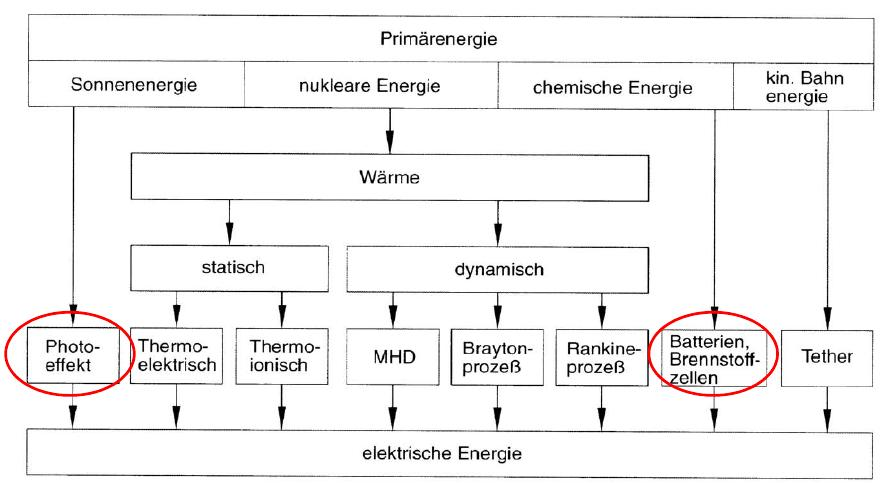
\includegraphics[scale=0.6]{energysources}
 \caption{Energy Sources}
\end{figure}
\begin{figure}[!ht]
 \centering
 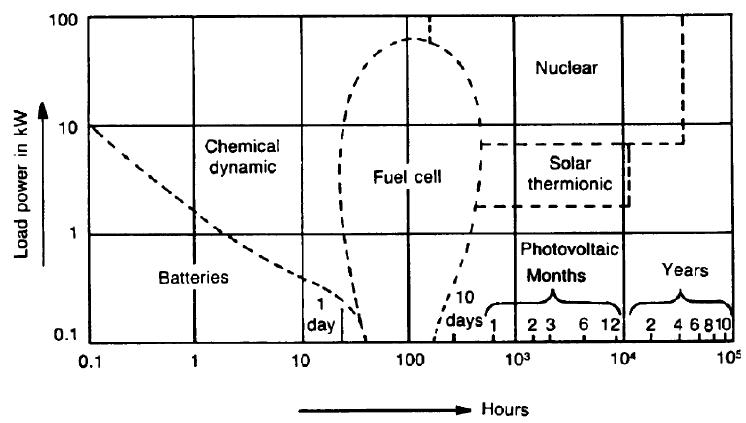
\includegraphics[scale=0.6]{energysourcesComparison}
 \caption{Comparison of Energy Sources}
\end{figure}

\subsection{Energy Storage}
 \begin{itemize}
  \item battery types: NiCD (no more used), NiH2 (mainly in telecommuniction satellites), Li-Ion (state of art), Li-Polymer (not yet used in space)
  \item fuel cells (ISS)
 \end{itemize}
\subsection{Source Control}
\begin{itemize}
 \item shunt regulator
 \item series regulator
 \item linear regulator
 \item peak power point tracker
\end{itemize}
\subsection{Main Requirements and Design Parameters}
\begin{itemize}
 \item average and peak power: determines the size of the solar array
 \item peak power: determines size of battery capacity
 \item battery charging: determines the solar array
 \item maximum discharge DoD: $< 40\%$ for Li-Ion
 \item mission lifetime: determines the degradation und subsequently sizing of battery and solar array
 \item orbit geometry: determines the available solar energy, radiation environment and eclipse durations
 \item solar constant: $1358 \frac{W}{m^2}$ mean above atmosphere. Seasonal variation: $1310-1400 \frac{W}{m^2}$
 \item satellite must be able to recover from total power loss without assistance from ground 
\end{itemize}

\subsection{Radiation Effects}
The following impacts on operation of electronic systems are associated with the charged particle environment:
\begin{itemize}
 \item TID (total ionization dose): degradation of electronics which result from proton and electron degradation in semiconductor devices
 \item SEL (single event latch-up): SELs occur when a single event causes a high current state. They may destroy the device, or they may be recoverable with a power-reset.
 \item SEB (single event burnout): heavy ion passes through a MOSFET (metal-oxide-semiconductor field-effect transistor). This induces a current flow which leads to device destruction 
 if sufficient short-circuit energy is available.
 \item SEU (single event upset): transients induced by charged particles that lose energy by ionizing the crystal lattice, leaving a wake of electron-hole pairs. The charged particles 
 usually arise from the radiation belts or from cosmic rays
\end{itemize}
\[\frac{\text{EOL}}{\text{BOL}} = \text{degradation}\]
\subsection{Efficiency and Degradation Consideration}
\begin{itemize}
 \item production efficiency $\eta$ of solar cells (14-22\%)
 \item path efficiency from solar array through batteries to loads: $X_e=0.65, X_d=0.85$ (direct energy transfer), $X_e=0.60, X_d=0.80$ (peak power tracking)
 \item inherent degradation: $I_d \approx 0.77$, ranges from $0.49-0.88$
 \item cosine loss, angle $\Theta$ between array normal and sun vector; typically use worst-case sun-angle
 \item life degradation: micrometeorites, radiation, etc. (2-4\% per year)\[L_d = (1-\text{degradation per year})^{\text{satellite life}}\]
\end{itemize}
\subsection{From Begin of Life to End of Life}
\[P_{o} = \eta\cdot 1358\frac{W}{m^2} \text{\qquad output power}\]
\[P_{BOL} = P_o\cdot I_d\cdot cos(\Theta)\]
\[P_{EOL} = L_d\cdot P_{BOL}\]
solar array size to meet power requirement:
\[A_{sa} = \frac{P_{sa}}{P_{EOL}}\]
mass of solar array ranges from $14$ to $47 \frac{W}{kg}$:
\[M_{sa} = 0.04\cdot P_{sa} \text{ \qquad (for } 25 \frac{W}{kg})\]
\subsection{Maximum Power Point Tracker (MPPT)}
\begin{itemize}
 \item continuously measures the power from the solar array and determines the maximum power point 
 \item adjusts the solar array interface voltage such that the actual power demand of the spacecraft can be delivered
 \item maximum efficiency ($>99\%$) can be achieved when the solar array interface voltage is close to the battery voltage
\end{itemize}
\subsection{Pros and Cons of Power Regulation}
\begin{itemize}
 \item power damper: excessive power will be absorbed in high power resistors, switch control system for resistors $\Rightarrow$ impact on thermal control system, as significant power 
 dissipation occurs 
 \item linear regulator: excessive power will be absorbed in high power transistor $\Rightarrow$ impact on thermal control system, as significant power dissipation occurs 
 \item shunt regulator: simple, robust, failsafe $\Rightarrow$ requires high number of cells per string to ensure battery charging and minimum power 
 \item MPPT: highest efficiency and minimum solar array size, complex in redundancy concept, each wing requires a dedicated MPPT
\end{itemize}
\subsection{Battery Sizing}
Power need:
\[P_{avg} = V_{bus}\cdot I\]
\[Ah_{avg} = \frac{T_e}{1h}\cdot I\]
\[Ah_{total} = \frac{Ah_{avg}}{DoD}\]
Capacity:
\[C_r = \frac{P_{avg}\cdot T_e}{DoD\cdot N_{bat} \cdot \eta}\]
\subsection{Power Distribution}
\begin{itemize}
 \item protection by fuse
 \item electronic protections
 \item limit current in failure case
 \item isolate failed components from bus
\end{itemize}
